\documentclass{article}[18pt]
\ProvidesPackage{format}
%Page setup
\usepackage[utf8]{inputenc}
\usepackage[margin=0.7in]{geometry}
\usepackage{parselines} 
\usepackage[english]{babel}
\usepackage{fancyhdr}
\usepackage{titlesec}
\hyphenpenalty=10000

\pagestyle{fancy}
\fancyhf{}
\rhead{Sam Robbins}
\rfoot{Page \thepage}

%Characters
\usepackage{amsmath}
\usepackage{amssymb}
\usepackage{gensymb}
\newcommand{\R}{\mathbb{R}}

%Diagrams
\usepackage{pgfplots}
\usepackage{graphicx}
\usepackage{tabularx}
\usepackage{relsize}
\pgfplotsset{width=10cm,compat=1.9}
\usepackage{float}

%Length Setting
\titlespacing\section{0pt}{14pt plus 4pt minus 2pt}{0pt plus 2pt minus 2pt}
\newlength\tindent
\setlength{\tindent}{\parindent}
\setlength{\parindent}{0pt}
\renewcommand{\indent}{\hspace*{\tindent}}

%Programming Font
\usepackage{courier}
\usepackage{listings}
\usepackage{pxfonts}

%Lists
\usepackage{enumerate}
\usepackage{enumitem}

% Networks Macro
\usepackage{tikz}


% Commands for files converted using pandoc
\providecommand{\tightlist}{%
	\setlength{\itemsep}{0pt}\setlength{\parskip}{0pt}}
\usepackage{hyperref}

% Get nice commands for floor and ceil
\usepackage{mathtools}
\DeclarePairedDelimiter{\ceil}{\lceil}{\rceil}
\DeclarePairedDelimiter{\floor}{\lfloor}{\rfloor}

% Allow itemize to go up to 20 levels deep (just change the number if you need more you madman)
\usepackage{enumitem}
\setlistdepth{20}
\renewlist{itemize}{itemize}{20}

% initially, use dots for all levels
\setlist[itemize]{label=$\cdot$}

% customize the first 3 levels
\setlist[itemize,1]{label=\textbullet}
\setlist[itemize,2]{label=--}
\setlist[itemize,3]{label=*}

% Definition and Important Stuff
% Important stuff
\usepackage[framemethod=TikZ]{mdframed}

\newcounter{theo}[section]\setcounter{theo}{0}
\renewcommand{\thetheo}{\arabic{section}.\arabic{theo}}
\newenvironment{important}[1][]{%
	\refstepcounter{theo}%
	\ifstrempty{#1}%
	{\mdfsetup{%
			frametitle={%
				\tikz[baseline=(current bounding box.east),outer sep=0pt]
				\node[anchor=east,rectangle,fill=red!50]
				{\strut Important};}}
	}%
	{\mdfsetup{%
			frametitle={%
				\tikz[baseline=(current bounding box.east),outer sep=0pt]
				\node[anchor=east,rectangle,fill=red!50]
				{\strut Important:~#1};}}%
	}%
	\mdfsetup{innertopmargin=10pt,linecolor=red!50,%
		linewidth=2pt,topline=true,%
		frametitleaboveskip=\dimexpr-\ht\strutbox\relax
	}
	\begin{mdframed}[]\relax%
		\centering
		}{\end{mdframed}}



\newcounter{lem}[section]\setcounter{lem}{0}
\renewcommand{\thelem}{\arabic{section}.\arabic{lem}}
\newenvironment{defin}[1][]{%
	\refstepcounter{lem}%
	\ifstrempty{#1}%
	{\mdfsetup{%
			frametitle={%
				\tikz[baseline=(current bounding box.east),outer sep=0pt]
				\node[anchor=east,rectangle,fill=blue!20]
				{\strut Definition};}}
	}%
	{\mdfsetup{%
			frametitle={%
				\tikz[baseline=(current bounding box.east),outer sep=0pt]
				\node[anchor=east,rectangle,fill=blue!20]
				{\strut Definition:~#1};}}%
	}%
	\mdfsetup{innertopmargin=10pt,linecolor=blue!20,%
		linewidth=2pt,topline=true,%
		frametitleaboveskip=\dimexpr-\ht\strutbox\relax
	}
	\begin{mdframed}[]\relax%
		\centering
		}{\end{mdframed}}
\lhead{CSys - OS}


\begin{document}
\begin{center}
\underline{\huge File - System Interface}
\end{center}
\section{File Concept}
\begin{itemize}
	\item Contiguous logical address space
	\item Types
	\begin{itemize}
		\item Data
		\begin{itemize}
			\item Numeric
			\item Character
			\item Binary
		\end{itemize}
		\item Program
	\end{itemize}
	\item Contents defined by file's creator
	\begin{itemize}
		\item Many types like text, source, executable 
	\end{itemize}
\end{itemize}
\section{File attributes}
\begin{itemize}
	\item \textbf{Name} - Only information kept in human-readable form
	\item \textbf{Identifier} - Unique tag (number) identifies file within file system
	\item \textbf{Type} - Needed for systems that support different types
	\item \textbf{Location} - Pointer to the file location on device
	\item \textbf{Size} - Current file size
	\item \textbf{Protection} - Controls who can do reading, writing, executing
	\item \textbf{Time, date and user id} - Data for protection, security and usage monitoring
	\item Information about files are kept in the directory structure, which is maintained on the disk
	\item Many variations, including extended file attributes such as file checksum
	\item Information kept in the directory structure
\end{itemize}
\section{File operations}
\begin{itemize}
	\item File is an abstract data type
	\item Create
	\item Write - At write pointer location
	\item Read - Ar read pointer location
	\item Reposition within file - seek
	\item Delete
	\item Truncate
	\item $Open(F_i)$ - search the directory structure on dis for entry $F_i$ and move the content of entry to memory
	\item $Close(F_i)$ - move the content of entry $F_i$ in memory to directory structure on disk
\end{itemize}
\section{Open files}
\begin{itemize}
	\item Several pieces of data are needed to manage open files:
	\begin{itemize}
		\item Open-file table - tracks open files
		\item File pointer: pointer to last read/write location, per process that has the file open
		\item File-open count: counter of number of times a file is open  - to allow removal of data from open-file table when last process closes it
		\item Disk location of the file: cache of data access information
		\item Access rights: per process access mode information
	\end{itemize}
\end{itemize}
\section{Open file locking}
\begin{itemize}
	\item Provided by some operating systems and file systems
	\begin{itemize}
		\item Similar to reader-writer locks
		\item Shared lock similar to reader lock - several process can acquire concurrently
		\item Exclusive lock similar to writer lock
	\end{itemize}
	\item Mediates access to a file
	\item Mandatory or advisory
	\begin{itemize}
		\item Mandatory - Access is denied depending on locks held and requested
		\item Advisory - Process can find status of locks and decide what to do
	\end{itemize}
\end{itemize}
\section{File structure}
\begin{itemize}
	\item None - sequence of words, bytes
	\item Simple record structure
	\begin{itemize}
		\item Lines
		\item Fixed length
		\item Variable length
	\end{itemize}
	\item Complex Structures
	\begin{itemize}
		\item Formatted document
		\item Relocatable load file
	\end{itemize}
	\item Can simulate last two with first method by inserting appropriate control characters
	\item Who decides
	\begin{itemize}
		\item Operating system
		\item Program
	\end{itemize}
\end{itemize}
\section{Sequential access file}
\begin{center}
	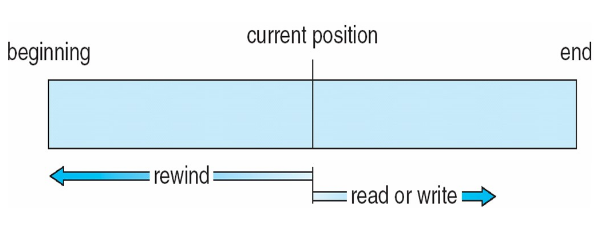
\includegraphics[scale=0.7]{sa}
\end{center}
\section{Access methods}
\begin{itemize}
	\item Sequential access
	\begin{center}
		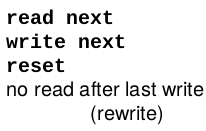
\includegraphics[scale=0.7]{sequential}
	\end{center}
	\item Direct access - file is fixed length logical records
	\begin{center}
		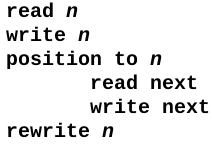
\includegraphics[scale=0.7]{direct}
	\end{center}
	\item Relative block numbers allow the OS to decide where the block should be placed
\end{itemize}
\section{Simulation of Sequential access on a direct-access file}
\begin{tabular}{|c|c|}
	\hline 
	Sequential Acess & Implementation for direct access \\ 
	\hline 
	Reset & cp=0; \\ 
	\hline 
	Read Next & read cp;\newline cp=cp+1; \\ 
	\hline 
	Write next & write cp;\newline cp=cp+1; \\ 
	\hline 
\end{tabular} 
\section{Other access methods}
\begin{itemize}
	\item Can be built on top of base methods
	\item General involve creation of an index for the file
	\item Keep index in memory for fast determination of location of data to be operated on (consider UPC code plus record of data about that item)
	\item If too large, index (in memory) of the index (on disk)
\end{itemize}
\begin{center}
	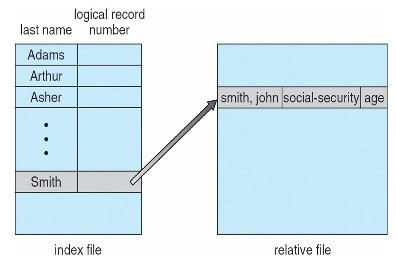
\includegraphics[scale=0.7]{database}
\end{center}
\section{Directory Structure}
\begin{itemize}
	\item A collection of nodes containing information about all files
	\begin{center}
		\includegraphics[scale=0.7]{"directory structure"}
	\end{center}
\end{itemize}
Both the directory structure and the files reside on disk
\section{Disk structure}
\begin{itemize}
	\item Disk can be subdivided into partitions
	\item Disks or partitions can be RAID protected against failure
	\item Disk or partition can be used raw - without a file system, or formatted with a file system
	\item Partitions also known as minidisks, slices
	\item Entity containing file system known as volume
	\item Each volume containing file system also tracks that file system's info in device directory or volume table of contents
	\item A well as general-purpose file systems there are many special-purpose file systems, frequently all within the same operating system or computer
\end{itemize}
\section{A Typical File-system Organization}
\begin{center}
	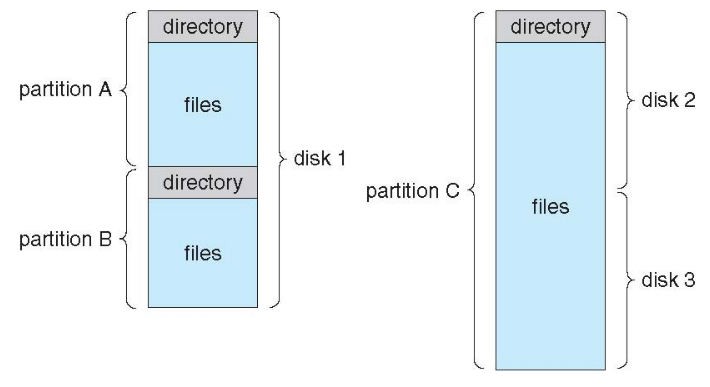
\includegraphics[scale=0.7]{Organisation}
\end{center}
\section{Operations Performed on Directory}
\begin{itemize}
	\item Search for a file
	\item Create a file
	\item Delete a file
	\item List a directory
	\item Rename a file
	\item Traverse the file system
\end{itemize}
\section{Directory Organisation}
The directory is organized logically to obtain
\begin{itemize}
	\item Efficiency - Locating a file quickly
	\item Naming - convenient to users
	\begin{itemize}
		\item Two users can have the same name for different files
		\item The same file can have several different names
	\end{itemize}
	\item Grouping - logical grouping of files by properties
\end{itemize}
\section{Single-Level Directory}
\begin{itemize}
	\item A single directory for all users
	\begin{center}
		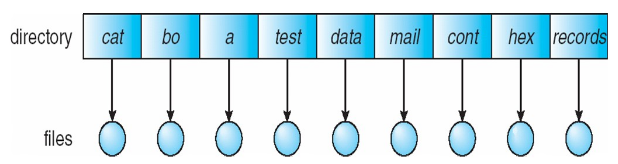
\includegraphics[scale=0.7]{single}
	\end{center}
	\item Naming problem
	\item Grouping problem
\end{itemize}
\section{Two level directory}
\begin{itemize}
	\item Separate directory for each user
	\begin{center}
		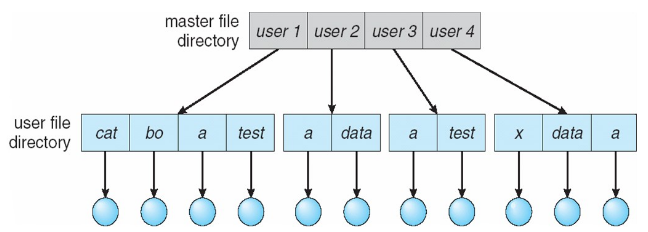
\includegraphics[scale=0.7]{two}
	\end{center}
	\item Path name
	\item Can have the same file name for different user
	\item Efficient searching
	\item No grouping capability
\end{itemize}
\section{Tree-Structured Directories}
\begin{center}
	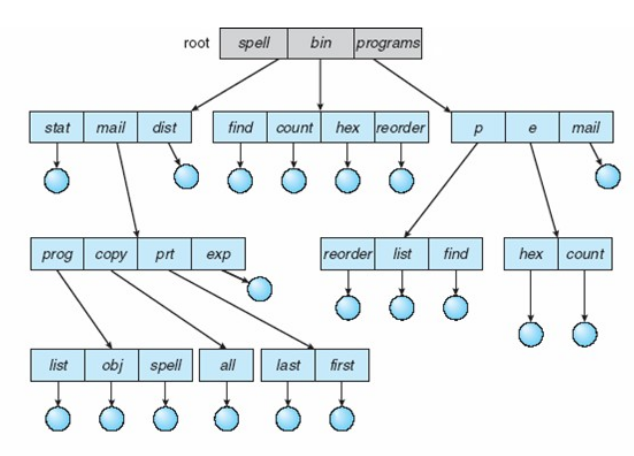
\includegraphics[scale=0.7]{tree}
\end{center}
\begin{itemize}
	\item Efficient searching
	\item Grouping capability
	\item Absolute or relative path name
	\item Creating a new file is done in current directory
\end{itemize}
\section{Acyclic-Graph Directories}
\begin{itemize}
	\item Have shared subdirectories and files
	\begin{center}
		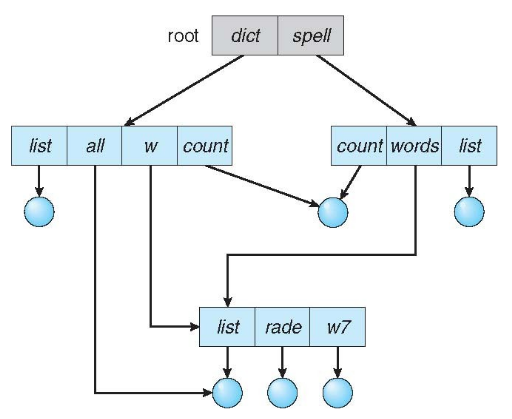
\includegraphics[scale=0.7]{acyclic}
	\end{center}
	\item Two different names (aliasing)
	\item If dict deletes list $\Rightarrow$ dangling pointer\\
	Solutions
	\begin{itemize}
		\item Backpointers, so we can delete all pointers. Variable size records a problem
		\item Backpointers using a daisy chain organization
		\item Entry-hold-count solution
	\end{itemize}
	\item New directory entry type
	\begin{itemize}
		\item Link - another name (pointer) to an existing file
		\item Resolve the link - follow pointer to locate the file
	\end{itemize}
\end{itemize}
\section{General Graph Directory}
\begin{center}
	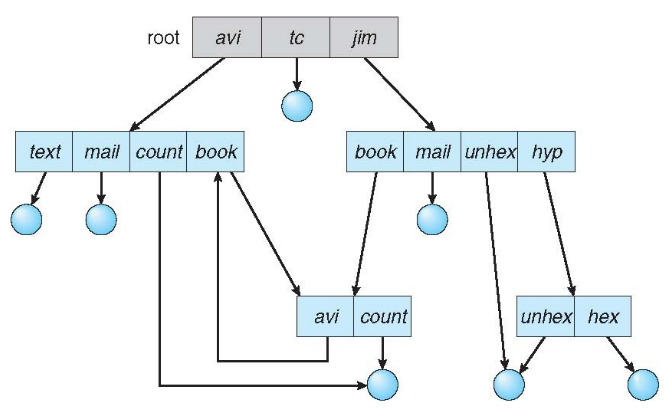
\includegraphics[scale=0.7]{General}
\end{center}
\begin{itemize}
	\item How do we guarantee no cycles?
	\begin{itemize}
		\item Allow only links to file not subdirectories
		\item Garbage collection
		\item Every time a new link is added use a cycle detection algorithm to determine whether it is OK
	\end{itemize}
\end{itemize}
\section{File Sharing}
\begin{itemize}
	\item Sharing of files on multi user systems is desirable
	\item Sharing may be done through a protection scheme
	\item On distributed systems, files may be shared across a network
	\item Network File Systems (NFS) is a common distributed file-sharing method
	\item If multi user system
	\begin{itemize}
		\item User IDs identify users, allowing permissions and protections to be per-user\\
		Group IDs allow users to be in groups, permitting group access rights
		\item Owner of a file/directory
		\item Group of a file/directory
	\end{itemize}
\end{itemize}
\subsection{Failure Modes}
\begin{itemize}
	\item All file systems have failure modes. For example, corruption of directory structures or other non-user data, called metadata
	\item Remote file systems add new failure modes, due to network failure, server failure
	\item Recovery from failure can involve state information about status of each remote request
	\item Stateless protocols such as NFS v3 include all information in each request, allowing easy recovery but less security
\end{itemize}
\subsection{Consistency Schematics}
\begin{itemize}
	\item Specify how multiple users are to access a shared file simultaneously
	\begin{itemize}
		\item Tend to be less complex due to disk I/O and network latency
		\item Andrew File System (AFS) implemented complex remote file sharing semantics
		\item Unix file system (UFS) implements:
		\begin{itemize}
			\item Writes to an open file visible immediately to other users of the same open file
			\item Sharing file pointer to allow multiple users to read and write concurrently
		\end{itemize}
		\item AFS has session semantics - Writes only visible to sessions starting after the file is closed
	\end{itemize}
\end{itemize}
\section{Protection}
\begin{itemize}
	\item File owner/creator should be able to control:
	\begin{itemize}
		\item What can be done
		\item By whom
	\end{itemize}
	\item Types of access
	\begin{itemize}
		\item Read
		\item Write
		\item Execute
		\item Append
		\item Delete
		\item List
	\end{itemize}
\end{itemize}
\subsection{Access Lists and Groups}
\begin{itemize}
	\item Mode of access: read, write, execute
	\item Three classes of users on Unix/ Linux
	\begin{center}
		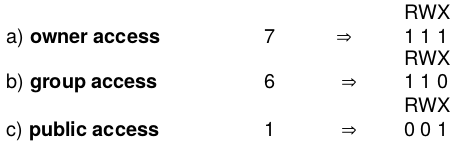
\includegraphics[scale=0.7]{users}
	\end{center}
	\item Ask manager to create a group (unique name), say G, and add some users to the group
	\item For a particular file (say game) or subdirectory, define an appropriate access
\end{itemize}
\begin{center}
	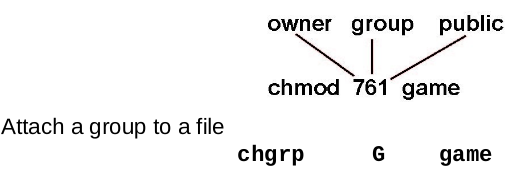
\includegraphics[scale=0.7]{group}
\end{center}

\end{document}